\documentclass[12pt,a4paper]{article}
\usepackage[utf8]{vietnam}
\usepackage{amsmath,amssymb}
\usepackage{geometry}
\geometry{top=1.5cm,bottom=1.2cm,left=1.4cm,right=1.4cm,headheight=28pt,headsep=12pt,footskip=18pt}
\usepackage{tikz}
\usepackage{xcolor}
\usepackage{enumerate}
\usepackage{graphicx}
\usepackage[version=4]{mhchem}
\usepackage{fancyhdr}
\usepackage{ex_test}

\renewcommand{\baselinestretch}{0.96}
\setlength{\parskip}{0pt}

\definecolor{hfRed}{RGB}{211,47,47}
\definecolor{hfGreen}{RGB}{139,195,144}

\providecommand{\False}{}

\pagestyle{fancy}
\fancyhf{}
\fancyhead[L]{\small\itshape\color{hfRed} Tài liệu lưu hành nội bộ}
\fancyhead[R]{\small\itshape\color{hfRed} Thầy \textbf{TRẦN VĂN THẠNH} - 0777.470.803}
\renewcommand{\headrulewidth}{0.8pt}
\renewcommand{\headrule}{\hbox to\headwidth{\color{hfGreen}\leaders\hrule height \headrulewidth\hfill}}

\fancyfoot[L]{\small\itshape\color{hfRed} CS1: 6/15 Nguyễn Hoàng, P. Kim Long, TP Huế \quad|\quad CS2: 24 Đặng Thái Thân, TP Huế}
\fancyfoot[R]{\small\bfseries\color{hfRed} Trang \thepage}
\renewcommand{\footrulewidth}{0.8pt}
\renewcommand{\footrule}{\hbox to\headwidth{\color{hfGreen}\leaders\hrule height \footrulewidth\hfill}}

\fancypagestyle{firstpage}{
  \fancyhf{}
  \renewcommand{\headrulewidth}{0pt}
  \fancyfoot[L]{\small\itshape\color{hfRed} CS1: 6/15 Nguyễn Hoàng, P. Kim Long, TP Huế \quad|\quad CS2: 24 Đặng Thái Thân, TP Huế}
  \fancyfoot[R]{\small\bfseries\color{hfRed} Trang \thepage}
  \renewcommand{\footrulewidth}{0.8pt}
  \renewcommand{\footrule}{\hbox to\headwidth{\color{hfGreen}\leaders\hrule height \footrulewidth\hfill}}
}

\begin{document}
\thispagestyle{firstpage}

\noindent
\begin{minipage}[t]{0.44\textwidth}
	\centering\fontsize{10pt}{12pt}\selectfont
	\textbf{SỞ GIÁO DỤC VÀ ĐÀO TẠO THỪA THIÊN HUẾ}\\
	\textbf{ĐỀ CHÍNH THỨC}\\
	\textit{(Đề thi có 04 trang)}
\end{minipage}\hfill
\begin{minipage}[t]{0.54\textwidth}
	\centering\small
	\textbf{ĐỀ KIỂM TRA ĐỊNH KỲ CHƯƠNG 2 (CARBOHYDRATE)}\\
	\textbf{MÔN: HOÁ HỌC -- LỚP 12}\\
	\textit{Thời gian làm bài: 50 phút (không kể thời gian phát đề)}\\
	\fbox{\textbf{MÃ ĐỀ: 104}}
\end{minipage}

\smallskip
\noindent\hrulefill
\smallskip

\noindent\textbf{Họ, tên thí sinh:} \dotfill\ \textbf{Lớp:} \dotfill\ \textbf{Số báo danh:} \dotfill

\smallskip
\noindent\textit{(Cho biết nguyên tử khối: H = 1; C = 12; N = 14; O = 16; Na = 23; K = 39; Cu = 64; Ag = 108).}

\vspace{0.2cm}
\noindent
\textbf{PHẦN I (4,5 điểm -- 18 câu): Câu trắc nghiệm nhiều phương án lựa chọn.}\\
\textit{Thí sinh trả lời từ câu 1 đến câu 18. Mỗi câu hỏi thí sinh chỉ chọn một phương án.}

\Opensolutionfile{ans}[ans-de04hs]

\begin{ex}
Đồng phân của glucose là
\choice
{fructose}
{tinh bột}
{saccharose}
{cellulose}
\loigiai{}
\end{ex}

\begin{ex}
Ứng dụng nào sau đây \textbf{không} phải là ứng dụng của glucose?
\choice
{Tráng gương, tráng phích}
{Nguyên liệu sản xuất chất dẻo PVC}
{Nguyên liệu sản xuất ethyl alcohol}
{Làm thực phẩm dinh dưỡng và thuốc tăng lực}
\loigiai{}
\end{ex}

\begin{ex}
Glucose là chất dinh dưỡng và được dùng làm thuốc tăng lực cho người già, trẻ em và người ốm. Số nguyên tử carbon trong phân tử glucose là
\choice
{6}
{11}
{5}
{12}
\loigiai{}
\end{ex}

\begin{ex}
(SBT -- CTST) Hormone nào sau đây làm giảm lượng glucose trong máu?
\choice
{Adrenaline}
{Thyroxine}
{Insuline}
{Oxytocine}
\loigiai{}
\end{ex}

\begin{ex}
(SBT -- KNTT) Phản ứng đặc trưng của maltose là
\choice
{Phản ứng với dung dịch $\ce{NaOH}$}
{Phản ứng màu với iodine}
{Phản ứng thuỷ phân tạo ra glucose}
{Phản ứng lên men trực tiếp tạo ra ethanol}
\loigiai{}
\end{ex}

\begin{ex}
(SBT -- KNTT) Saccharose và maltose đều tham gia phản ứng nào sau đây?
\choice
{Phản ứng với thuốc thử Tollens}
{Phản ứng thuỷ phân trong môi trường acid}
{Phản ứng với dung dịch nước bromine}
{Phản ứng với $\ce{Cu(OH)2}$ tạo kết tủa đỏ gạch}
\loigiai{}
\end{ex}

\begin{ex}
(SBT -- KNTT) Cellulose \textbf{không} được sử dụng trong ứng dụng nào sau đây?
\choice
{Sản xuất các thiết bị điện}
{Nguyên liệu sản xuất ethanol và cellulose nitrate}
{Sản xuất giấy, tơ tự nhiên và sợi nhân tạo}
{Vật liệu gỗ xây dựng}
\loigiai{}
\end{ex}

\begin{ex}
(SBT -- KNTT) Nguyên liệu nào sau đây \textbf{không} phải là nguồn cung cấp tinh bột?
\choice
{Củ và quả}
{Hạt ngũ cốc}
{Sợi bông}
{Gạo}
\loigiai{}
\end{ex}

\begin{ex}
(SGK -- CD) Nhận xét nào dưới đây là \textbf{không đúng} khi nói về glucose và fructose?
\choice
{Đều tạo được dung dịch màu xanh lam khi tác dụng với $\ce{Cu(OH)2}$ trong môi trường kiềm}
{Đều tạo được kết tủa đỏ gạch $\ce{Cu2O}$ khi tác dụng với $\ce{Cu(OH)2}$, đun nóng trong môi trường kiềm}
{Đều làm mất màu nước bromine}
{Đều xảy ra phản ứng tráng bạc khi tác dụng với thuốc thử Tollens}
\loigiai{}
\end{ex}

\begin{ex}
(SGK 12 -- CTST) Carbohydrate nào dưới đây \textbf{không} có nhóm $-\ce{OH}$ hemiacetal hoặc nhóm $-\ce{OH}$ hemiketal?
\choice
{Glucose}
{Fructose}
{Saccharose}
{Maltose}
\loigiai{}
\end{ex}

\begin{ex}
(SBT -- CD) Polysaccharide mạch phân nhánh, có nhiều trong các loại ngũ cốc, thường được sử dụng làm lương thực là
\choice
{cellulose}
{amylose}
{amylopectin}
{glycogen}
\loigiai{}
\end{ex}

\begin{ex}
\def\dotEX{}
Công thức cấu tạo dạng mạch vòng $\beta$-glucose là
\choice
{\parbox[c]{3.5cm}{\centering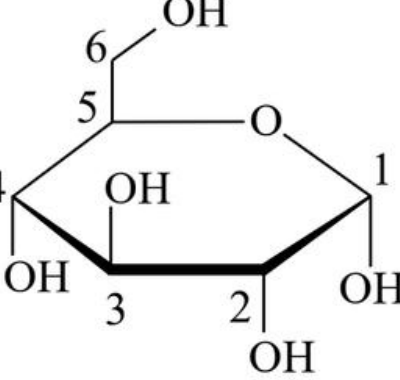
\includegraphics[height=1.8cm]{images_crop_de04/cau12_opt_A.png}}}
{\parbox[c]{3.5cm}{\centering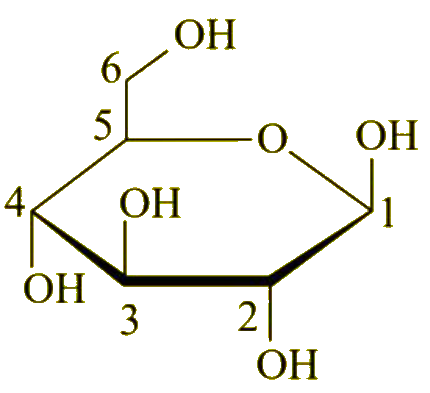
\includegraphics[height=1.8cm]{images_crop_de04/cau12_opt_B.png}}}
{\parbox[c]{3.5cm}{\centering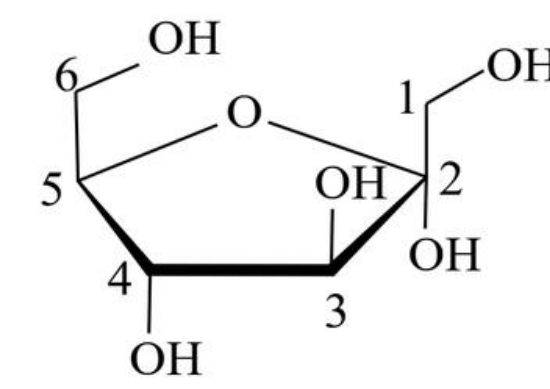
\includegraphics[height=1.8cm]{images_crop_de04/cau12_opt_C.png}}}
{\parbox[c]{3.5cm}{\centering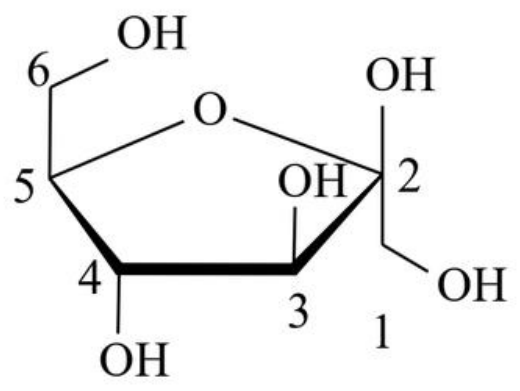
\includegraphics[height=1.8cm]{images_crop_de04/cau12_opt_D.png}}}
\def\dotEX{.}
\loigiai{}
\end{ex}

\begin{ex}
Chất T có các đặc điểm: (1) thuộc loại monosaccharide; (2) có nhiều trong quả nho chín; (3) tác dụng với nước bromine; (4) có phản ứng tráng gương. Chất T là
\choice
{glucose}
{saccharose}
{fructose}
{cellulose}
\loigiai{}
\end{ex}

\begin{ex}
Dãy các chất nào dưới đây đều phản ứng được với $\ce{Cu(OH)2}$ ở điều kiện thường?
\choice
{Ethylene glycol, glycerol và ethyl alcohol}
{Glucose, glycerol và saccharose}
{Glucose, glycerol và methyl acetate}
{Glycerol, glucose và ethyl acetate}
\loigiai{}
\end{ex}

\begin{ex}
Phương trình: $6n\ce{CO2} + 5n\ce{H2O} \xrightarrow[\text{chlorophyll}]{\text{asmt}} (\ce{C6H10O5})_n + 6n\ce{O2}$ là phản ứng hoá học chính của quá trình nào sau đây?
\choice
{quá trình hô hấp}
{quá trình quang hợp}
{quá trình khử}
{quá trình oxi hoá}
\loigiai{}
\end{ex}

\begin{ex}
Thí nghiệm: Phản ứng của glucose với $\ce{Cu(OH)2}$ khi đun nóng\\
\textit{Bước 1:} Cho khoảng 2 mL dung dịch $\ce{NaOH}$ 10\% vào ống nghiệm.\\
\textit{Bước 2:} Sau đó, thêm khoảng 0,5 mL dung dịch $\ce{CuSO4}$ 5\% vào, lắc nhẹ.\\
\textit{Bước 3:} Cho tiếp khoảng 3 mL dung dịch glucose 2\% vào ống nghiệm và lắc đều. Đun nóng ống nghiệm bằng ngọn lửa đèn cồn trong vài phút.\\
Phát biểu nào sau đây \textbf{sai}?
\choice
{Sản phẩm hữu cơ thu được sau bước 3 là sodium gluconate}
{Nếu thay dung dịch $\ce{NaOH}$ ở bước 2 bằng dung dịch $\ce{KOH}$ thì hiện tượng ở bước 3 vẫn tương tự}
{Thí nghiệm trên chứng minh glucose có tính chất của polyalcohol}
{Ở bước 3, nếu thay glucose bằng fructose thì hiện tượng xảy ra vẫn tương tự}
\loigiai{}
\end{ex}

\begin{ex}
Cho các phát biểu sau:\\
(a) Ở điều kiện thường, saccharose đều là chất rắn, dễ tan trong nước.\\
(b) Saccharose bị hóa đen khi tiếp xúc với sulfuric acid đặc.\\
(c) Trong công nghiệp dược phẩm, saccharose được dùng để pha chế thuốc.\\
(d) Thủy phân hoàn toàn saccharose chỉ thu được glucose.\\
Số phát biểu đúng là
\choice
{3}
{1}
{4}
{2}
\loigiai{}
\end{ex}

\begin{ex}
Cho các phát biểu sau:\\
(a) Có thể dùng nước bromine để phân biệt glucose và fructose.\\
(b) Trong môi trường acid, glucose và fructose có thể chuyển hoá lẫn nhau.\\
(c) Có thể phân biệt glucose và fructose bằng phản ứng với dung dịch $\ce{AgNO3}$ trong $\ce{NH3}$.\\
(d) Trong dung dịch, glucose và fructose đều hoà tan $\ce{Cu(OH)2}$ ở nhiệt độ thường cho dung dịch màu xanh lam.\\
(e) Trong dung dịch, fructose tồn tại chủ yếu ở dạng mạch hở.\\
(g) Trong dung dịch, glucose tồn tại chủ yếu ở dạng vòng 6 cạnh (dạng $\alpha$ và $\beta$).\\
Số phát biểu đúng là
\choice
{4}
{3}
{5}
{2}
\loigiai{}
\end{ex}

\Closesolutionfile{ans}

\vspace{0.3cm}
\noindent
\textbf{PHẦN II (4,0 điểm -- 4 câu): Câu trắc nghiệm đúng sai.}\\
\textit{Thí sinh trả lời từ câu 1 đến câu 4. Trong mỗi ý a), b), c), d) ở mỗi câu, thí sinh chọn đúng hoặc sai.}

\setcounter{ex}{0}

\begin{ex}
Một học sinh tiến hành làm thí nghiệm tráng bạc của glucose theo hai bước sau:\\
\textit{Bước 1:} Cho vào một ống nghiệm sạch 1 mL dung dịch $\ce{AgNO3}$ 1\%, sau đó nhỏ tiếp từng giọt dung dịch $\ce{NH3}$ vào cho đến khi kết tủa vừa xuất hiện lại tan hết.\\
\textit{Bước 2:} Thêm tiếp 1 mL dung dịch glucose 1\% vào ống nghiệm trên rồi đun nóng nhẹ.
\choiceTF[t]
{Phản ứng xảy ra ở bước 2 là: $\ce{CH2OH-[CHOH]4-CHO + 2AgNO3 + 3NH3 + H2O ->[t^\circ] CH2OH-[CHOH]4-COONH4 + 2Ag + 2NH4NO3}$}
{Hiện tượng xảy ra ở bước 2 là xuất hiện kết tủa màu đen}
{Ở bước 2 chất oxi hóa là glucose, chất khử là $\ce{AgNO3}$}
{Trong công nghiệp, người ta dùng sucrose làm nguyên liệu để tráng ruột phích mà không dùng glucose là vì sucrose có lượng nhiều trong tự nhiên, giá thành thấp đồng thời khi thủy phân sinh ra glucose và fructose đều có phản ứng tráng bạc còn glucose có lượng ít trong tự nhiên, giá thành cao}
\loigiai{}
\end{ex}

\begin{ex}
Hợp chất saccharose và maltose là chất rắn có vị ngọt, dễ tan trong nước.
\begin{center}
	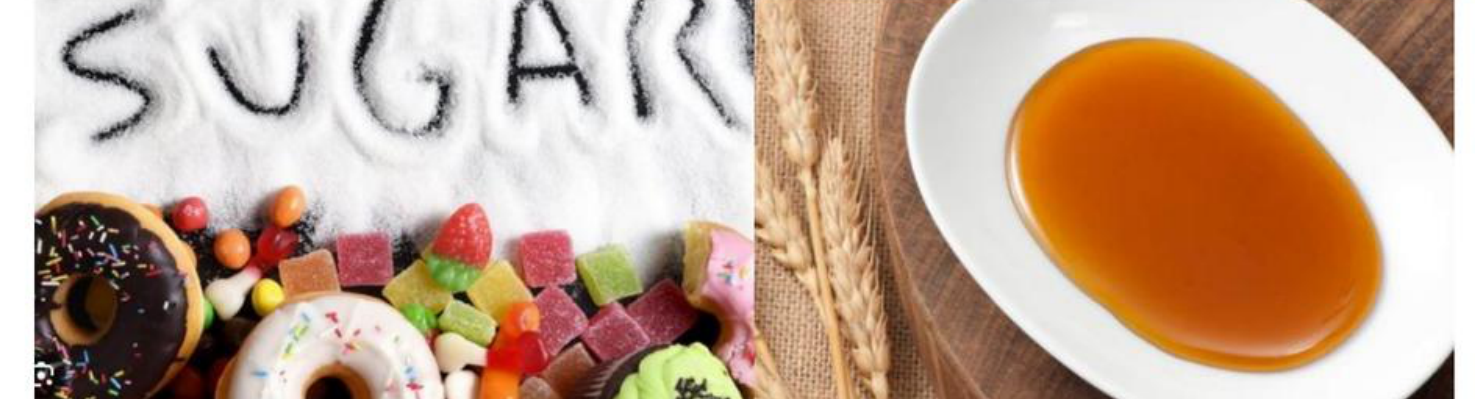
\includegraphics[width=9cm]{images_crop_de04/p2_cau2_sugar.png}
\end{center}
\choiceTF[t]
{Đều thuộc loại carbohydrate}
{Là hai chất đồng phân}
{Khi bị thủy phân hoàn toàn, mỗi phân tử đều tạo thành hai phân tử glucose}
{Đều thuộc loại disaccharide}
\loigiai{}
\end{ex}

\begin{ex}
Tinh bột là một polysaccharide gồm nhiều gốc $\alpha$-glucose liên kết với nhau tạo ra hai dạng mạch amylose và amylopectin, dưới đây là cấu tạo của một trong hai dạng này.
\begin{center}
	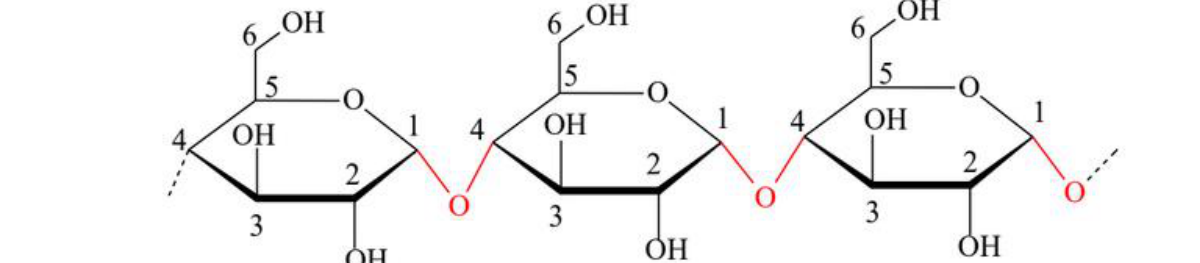
\includegraphics[width=12cm]{images_crop_de04/p2_cau3_amylose.png}
\end{center}
\choiceTF[t]
{Đoạn mạch trên là cấu tạo của dạng amylose trong tinh bột}
{Các gốc $\alpha$-glucose trong đoạn mạch trên liên kết với nhau bởi liên kết $\alpha$-1,6-glycoside}
{Công thức mỗi gốc $\alpha$-glucose là $\ce{C6H10O5}$}
{Đoạn mạch trên có cấu tạo phân nhánh ở liên kết $\alpha$-1,6-glycoside}
\loigiai{}
\end{ex}

\begin{ex}
Tính tan của cellulose trong nước Schweizer\\
\textit{Chuẩn bị:}\\
Hoá chất: cellulose (bông), dung dịch $\ce{CuSO4}$ 1 M, dung dịch $\ce{NaOH}$ 20\%, dung dịch $\ce{NH3}$ đặc.\\
Dụng cụ: giấy lọc, cốc thuỷ tinh 250 mL, đũa thuỷ tinh, ống hút.\\
\textit{Tiến hành:}\\
\textit{Bước 1:} Cho khoảng 50 mL dung dịch $\ce{CuSO4}$ 1 M vào cốc 250 mL. Thêm 20 mL dung dịch $\ce{NaOH}$ 20\% vào, khuấy đều.\\
\textit{Bước 2:} Lọc tách kết tủa, cho vào cốc thuỷ tinh 250 mL. Thêm khoảng 50 mL dung dịch $\ce{NH3}$ đặc, khuấy đều đến khi kết tủa tan hết thu được nước Schweizer.\\
\textit{Bước 3:} Thêm một lượng nhỏ bông vào khoảng 30 mL nước Schweizer và khuấy đều trong khoảng 3 phút.
\choiceTF[t]
{Sau bước 1, sản phẩm thu được là kết tủa $\ce{Cu(OH)2}$ có màu xanh}
{Ở bước 2 xảy ra phương trình tạo nước Schweizer như sau: $\ce{Cu(OH)2 + 4NH3 -> [Cu(NH3)4](OH)2}$ (Tetraamminecopper(II) hydroxide)}
{Sau bước 3, dung dịch thu được có sự phân lớp}
{Thí nghiệm trên chứng minh trong cellulose có 3 nhóm OH tự do}
\loigiai{}
\end{ex}

\vspace{0.3cm}
\noindent
\textbf{PHẦN III (1,5 điểm -- 6 câu): Câu trắc nghiệm yêu cầu trả lời ngắn.}\\
\textit{Thí sinh trả lời từ câu 1 đến câu 6. Mỗi câu hỏi thí sinh điền câu trả lời ngắn gọn theo yêu cầu.}

\setcounter{ex}{0}

\begin{ex}
Cho dãy các chất sau: saccharose, glucose, fructose, cellulose, tristearin, methyl acetate. Số chất tham gia phản ứng thuỷ phân là bao nhiêu?
\loigiai{}
\noindent\textbf{Đáp số:} \dotfill
\end{ex}

\begin{ex}
Cho các chất: saccharose, glucose, fructose, ethyl formate, formic acid và acetic aldehyde. Trong các chất trên, số chất vừa có khả năng tham gia phản ứng tráng bạc vừa có khả năng phản ứng với $\ce{Cu(OH)2}$ ở điều kiện thường là
\loigiai{}
\noindent\textbf{Đáp số:} \dotfill
\end{ex}

\begin{ex}
Cho dãy các chất sau: glucose, fructose, saccharose, cellulose, tinh bột. Số chất khi bị thủy phân trong môi trường acid chỉ tạo glucose là
\loigiai{}
\noindent\textbf{Đáp số:} \dotfill
\end{ex}

\begin{ex}
Để tráng một số lượng gương soi có diện tích bề mặt $0{,}35\text{ m}^2$ với độ dày $0{,}1\ \mu\text{m}$ người ta đun nóng dung dịch chứa $26{,}77\text{ gam}$ glucose với một lượng dung dịch silver nitrate trong ammonia. Biết khối lượng riêng của silver là $10{,}49\text{ g/cm}^3$, hiệu suất phản ứng tráng gương là $80\%$ (tính theo glucose). Số lượng gương soi tối đa sản xuất được khoảng bao nhiêu?
\loigiai{}
\noindent\textbf{Đáp số:} \dotfill
\end{ex}

\begin{ex}
Tại một nhà máy rượu, cứ $10\text{ tấn}$ tinh bột (chứa $6{,}85\%$ tạp chất trơ) sẽ sản xuất được $7{,}21\text{ m}^3$ ethanol $40^\circ$ (cho khối lượng riêng của ethanol nguyên chất là $0{,}789\text{ g/cm}^3$). Hiệu suất của quá trình sản xuất là $H\%$. Xác định giá trị của $H$ (làm tròn một chữ số thập phân).
\begin{center}
	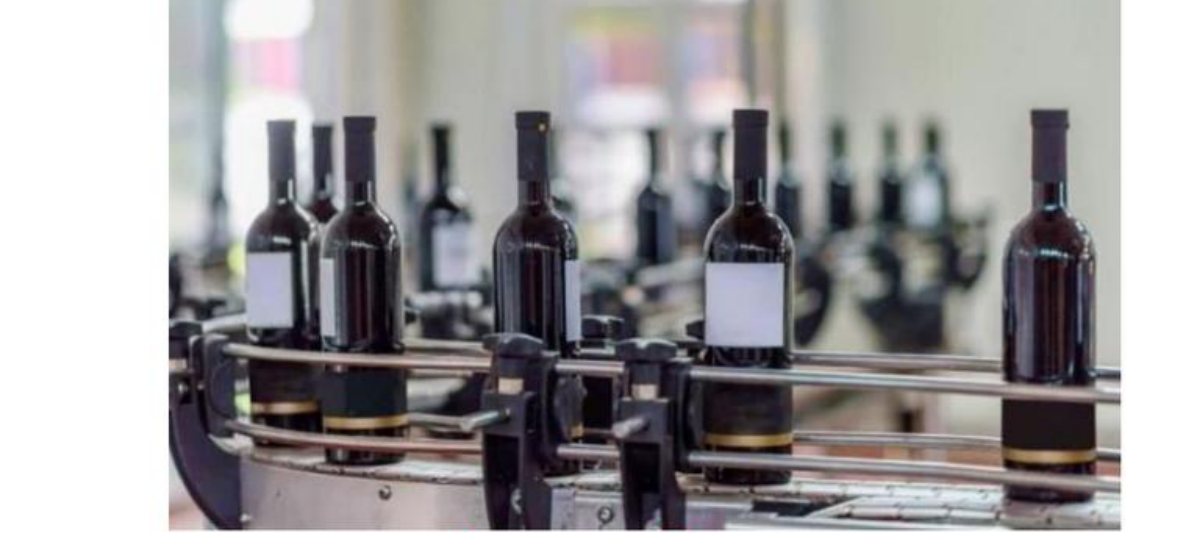
\includegraphics[width=9cm]{images_crop_de04/p3_cau5_wine.png}\\
	\textit{\small\color{hfRed} Dây chuyền sản xuất rượu (alcohol)}
\end{center}
\loigiai{}
\noindent\textbf{Đáp số:} \dotfill
\end{ex}

\begin{ex}
(SBT -- CD) Theo Tiêu chuẩn Việt Nam TCVN 7624:2007, khi chế tạo gương, chiều dày lớp bạc phủ trên bề mặt tấm kính (quy ra tổng lượng bạc trên một đơn vị $\text{m}^2$ kính) phải đạt tối thiểu $0{,}7\text{ g}\cdot\text{m}^{-2}$. Một công ty cần sản xuất $10000\text{ m}^2$ gương có độ dày lớp bạc phủ ở mức $0{,}72\text{ g}\cdot\text{m}^{-2}$. Biết rằng lớp bạc được tạo thành qua phản ứng giữa silver nitrate và glucose trong điều kiện thích hợp với hiệu suất phản ứng $90\%$. Khối lượng glucose cần sử dụng để sản xuất $10000\text{ m}^2$ gương trên là bao nhiêu kg? (Làm tròn đến chữ số thập phân thứ hai).
\loigiai{}
\noindent\textbf{Đáp số:} \dotfill
\end{ex}


\begin{center}
	\textbf{---------- HẾT ----------}
\end{center}

\end{document}
